\documentclass{classrep}
\usepackage[utf8]{inputenc}
\usepackage{color}
\usepackage{makecell}
\usepackage{graphicx}
\usepackage{url}
\usepackage{hyperref}

\studycycle{Informatyka, studia STACJONARNE, I st.}
\coursesemester{VI}

\coursename{Komputerowe systemy rozpoznawania}
\courseyear{2020/2021}

\courseteacher{prof. dr hab. inż. Adam Niewiadomski}
\coursegroup{poniedziałek, 12:00}

\author{
  \studentinfo{Julia Szymańska}{224441} \and
  \studentinfo{Przemysław Zdrzalik}{224466} }

\title{Projekt 1. Klasyfikacja dokumentów tekstowych}
\usepackage{multirow}
\begin{document}
\maketitle


%%%%%%%%%%%%%%%%%%%%%%%%%%%%%%%%%%%%%%%%%%%%%%%%%%%%%%%%%%%%%%%%%%
\section{Cel projektu}

Celem projektu jest stworzenie aplikacji klasyfikującej zadany zbiór danych tekstowych metodą K najbliższych sąsiadów (k-NN). Aplikacja ma za zadanie dokonać ekstrakcji cech na zbiorach tekstów\cite{dane} oraz następnie dokonać ich klasyfikacji.\\


%%%%%%%%%%%%%%%%%%%%%%%%%%%%%%%%%%%%%%%%%%%%%%%%%%%%%%%%%%%%%%%%%%
\section{Klasyfikacja nadzorowana metodą $k$-NN}

Metoda K najbliższych sąsiadów, w skrócie metoda $k$-NN\cite{dane}, jest to algorytm stosowany do klasyfikacji, który nie wymaga etapu uczenia. 
Polega na zaklasyfikowaniu rozpatrywanego elementu do grupy ze zbioru uczącego, gdzie spośród k najbliższych rozpatrywanemu elementowi sąsiadów najwięcej z nich należy do tej grupy. Klasyfikator przyjmuje cztery parametry wejściowe takie jak: warotść k - liczba rozpatrywanych sąsiadów, proporcje podziału zbiorów na zbior uczący i zbiór testowy, zbiór cech, a także metrykę i/lub miarę prawdopodobieństwa. Wynikiem klasyfikacji jest zaklasyfikowanie elementu do jednego ze zbiorów uczących. 


%%%%%%%%%%%%%%%%%%%%%%%%%%%%%%%%%%%%%%%%%%%%%%%%%%%%%%%%%%%%%%%%%%
\subsection{Ekstrakcja cech, wektory cech}

Na zbiorach danych tekstowych należy dokonać ekstrakcji cech, które będą wartościami rzeczywistymi oraz tekstowymi. Dane cechy będą reprezentowały tekst w postaci wektora cech podczas procesu klasyfikacji. Przed dokonaniem ekstrakcji cech, z tekstów usuwane są słowa znajdujące się na stop liście. Teksty ze zbioru danych tekstowych posiadają strukturę: \begin{equation}
  \begin{array}{l}
  <TEXT> \\
\;\;\;\; <TITLE/>\\
\;\;\;\; <AUTHOR/>\\
\;\;\;\; <DATELINE/>\\
 \;\;\;\;<BODY/> \\
</TEXT>
  \end{array}
\end{equation}\\
\begin{enumerate}
  \item Liczba słów - cecha ta oznacza liczbę słów które składają się na pobrany tekst. Cecha ta będzie charakteryzowała długość dokumentu w postaci liczby całkowitej \begin{equation}  c_1 = len \end{equation} gdzie len - liczba słów w tekście.\\
 \item Data z tagu  \textless Dateline\textgreater\ - Każdy tekst w swoim body posiada tag \textless Dateline\textgreater , w którym znajduje się miasto oraz data podana w postaci miesiąca i dnia. Data będzie konwertowana na wartość liczbową, gdzie liczbą tą będzie numer podanego dnia w ciągu roku, licząc rok tak jakby rok był rokiem przestępnym, przykładowo data 1 marca będzie reprezentowana poprzez wartość 61. Cechę traktujemy jako cechę w postaci liczby całkowitej. Wartość będzie oznaczana poprzez symbol  c\textsubscript{2}.    \\
  \item Lokacja z tagu \textless Dateline\textgreater - jak wyżej. Lokację traktujemy jako cechę tekstową. Wartość będzie oznaczana poprzez symbol  c\textsubscript{3}. \\
  \item Tytuł z tagu \textless Title\textgreater - Każdy tekst w swoim body posiada tag \textless Title\textgreater. Tytuł traktujemy jako cechę tekstową. Wartość będzie oznaczana poprzez symbol  c\textsubscript{4}.\\
  \item Autor z tagu \textless Author\textgreater - Większość tekstów w swoim body posiada tag \textless Author\textgreater. Autora traktujemy jako cechę tekstową. Wartość będzie oznaczana poprzez symbol  c\textsubscript{5}.\\
  \item Najczęściej występująca nazwa kraju - wybieramy najczęściej występującą w analizowanym tekście nazwę kraju. Nazwy krajów pobieramy z dołączonego pliku all-places-strings.lc, przykładowo krajem występującym w pliku jest 'albania'.Nazwę kraju traktujemy jako cechę tekstową.Wartość będzie oznaczana poprzez symbol  c\textsubscript{6}.\\
  \item Zbiór występujących słów kluczowych. Za słowa kluczowe przyjmujemy słowa znajdujące się w dołączonych plikach o rozszerzeniach .lc.txt. Cechę traktujemy jako cechę tekstową.  \begin{equation}  c_7 : c_7 \in N \cap t \end{equation} gdzie N - zbiór wszystkich słów kluczowych, t - zbiór słów należących do tekstu\\
  \item Liczba wystąpień słów kluczowych - traktujemy jako cechę w postaci liczby całkowitej.\begin{equation}  c_8 = | c_7 | \end{equation} gdzie c\textsubscript{8} - zbiór występujących słów kluczowych\\
  \item Nasycenie tekstu ilością słów kluczowych - traktujemy jako cechę w postaci liczby zmienno przecinkowej.  \begin{equation} c_{9} = c_8 / c_1 \end{equation}  gdzie c\textsubscript{9} - liczba wystąpień słów kluczowych w tekscie, c\textsubscript{1} - liczba słów w tekście\\
  \item Najczęściej występujące słowo kluczowe - wybieramy najczęściej występujące w analizowanym tekście słowo kluczowe. Cechę traktujemy jako cechę tekstową. Wartość będzie oznaczana poprzez symbol  c\textsubscript{10}.\\
  \item Liczba unikatowych słów - zliczamy liczbę unikatowych słów, to znaczy występujących dokładnie raz w analizowanym tekście. Cechę traktujemy jako cechę w postaci liczby całkowitej. Wartość będzie oznaczana poprzez symbol  c\textsubscript{11}.\\
\end{enumerate}


\ \\ \\
Wektor cech będzie reprezentowany w postaci: 

\begin{equation} w = [c_1, c_2, c_3, c_4, c_5, c_6, c_7, c_8, c_9, c_{10}, c_{11}] \end{equation}


%%%%%%%%%%%%%%%%%%%%%%%%%%%%%%%%%%%%%%%%%%%%%%%%%%%%%%%%%%%%%%%%%%
\subsection{Miary jakości klasyfikacji} 

W celu określenia jakości wykonanej klasyfikacji korzystamy z czterech miar jakości klasyfikacji. Aby obliczyć każdą z miar tworzymy tablicę pomyłek, inaczej macierz błędu \cite{tablica}. Tablica składa się z dwóch wierszy i dwóch kolumn, gdzie wiersze to klasy predykowane, a kolumny to klasy rzeczywiste. Dane oznaczone jako dane pozytywne i negatywne poddawane są klasyfikacji, która przypisuje im predykowaną klasę pozytywną bądź negatywną.\\

\begin{table}[h!]
\begin{tabular}{l|l|c|c|c}
\multicolumn{2}{c}{}&\multicolumn{2}{c}{Klasa rzeczywista}&\\
\cline{3-4}
\multicolumn{2}{c|}{}&Pozytywna&Negatywna&\multicolumn{1}{c}{}\\
\cline{2-4}
\multirow{2}{*}{\thead{Klasa\\ predykowana} }& Pozytywna&  \thead{prawdziwie\\ pozytywna (TP)}
 & \thead{fałszywie\\ pozytywna (FP)} \\
\cline{2-4}
& Negatywna & \thead{fałszywie\\ negatywna (FN)} & \thead{prawdziwie\\ negatywna (TN)} \\
\cline{2-4}
\end{tabular}
 \caption{Wzór tablicy pomyłek\cite{tablica}.}
\end{table}

We wzorach zostały użyte oznaczenia:
\begin{itemize}
\item TP - sumaryczna liczba poprawnie zaklasyfikowanych tekstów rozpatrywanej klasy 
\item TN - sumaryczna liczba poprawnie zaklasyfikowanych tekstów pozostałych klas
\item FP - sumaryczna liczba tekstów pozostałych klas zaklasyfikowanych do rozpatrywanej klasy
\item FN - sumaryczna liczba tekstów rozpatrywanej klasy zaklasyfikowanych do pozostałych klas
\end{itemize}

\ \\ \\ 
Stosowane miary jakości klasyfikacji:\\
\begin{itemize}
  \item Dokładność (ang. accuracy), ACC  - jest to stosunek poprawnie zaklasyfikowanych tekstów do wszystkich klasyfikowanych tekstów.
 \begin{equation}ACC = \frac{TP + TN}{TP + TN + FP + FN} \end{equation}
 \item Precyzja (ang. precision), PPV  - jest to stopień zgodności wyników uzyskanych w określonych warunkach z wielokrotnych pomiarów. Precyzja to stosunek liczby poprawnie zaklasyfikowanych tekstów rozpatrywanej klasy do liczby wszystkich tekstów zaklasyfikowanych do rozpatrywanej klasy. 
\begin{equation} PPV =  \frac{TP} {TP+FP} \end{equation} 
Dla całego zbioru dokumentów wartość miary jest liczona jako średnia ważona obliczonych precyzji dla pojedyńczych klas, gdzie wagą jest stosunek liczebności tej klasy do liczebności wszystkich klas. 
\begin{equation} PPV_{calk} = \sum_{n=1}^{m} (PPV_n *\frac{k_n}{k}) \end{equation}
Gdzie \textit{PPV\textsubscript{calk}} - precyzja obliczona dla wszystkich klas klasyfikowanych dokumentów,  \textit{m} - liczba rozpatrywanych klas, \textit{PPV\textsubscript{n}} - precyzja dla n-tej klasy, \textit{k\textsubscript{n}} - liczebność rzeczywista dokumentów klasy n, \textit{k} - liczebność wszystkich klasyfikowanych dokumentów\\
\item Czułość (ang. recall), TPR  - jest to stosunek liczby poprawnie zaklasyfikowanych tekstów do rozpatrywanej klasy do liczby tekstów z rozpatrywanej klasy. 
 \begin{equation}   TPR = \frac{TP}{TP + FN} \end{equation}
Dla całego zbioru dokumentów wartość miary jest liczona jako średnia ważona obliczonych czułości dla pojedyńczych klas, gdzie wagą jest stosunek liczebności tej klasy do liczebności wszystkich klas. 
\begin{equation} TPR_{calk} = \sum_{n=1}^{m} (TPR_n *\frac{k_n}{k}) \end{equation}
Gdzie \textit{TPR\textsubscript{calk}} - czułość obliczona dla wszystkich klas klasyfikowanych dokumentów,  \textit{m} - liczba rozpatrywanych klas, \textit{TPR\textsubscript{n}} - czułość dla n-tej klasy,  \textit{k\textsubscript{n}} - liczebność rzeczywista dokumentów klasy n, \textit{k} - liczebność wszystkich klasyfikowanych dokumentów\\
\item Miara F1 - średnia harmoniczna miar Precyzja i Czułość. 
\begin{equation}   F1 = \frac{2}{\frac{1}{PPV} + \frac{1}{TPR}} \end{equation}
\end{itemize}


%%%%%%%%%%%%%%%%%%%%%%%%%%%%%%%%%%%%%%%%%%%%%%%%%%%%%%%%%%%%%%%%%%
\section{Klasyfikacja z użyciem metryk i miar podobieństwa tekstów}

W procesie klasyfikacji możliwe jest wykorzystanie jednej z trzech metryk: metryka Euklidesowa, metryka Czebyszewa, metryka Uliczna. Metryki służą obliczeniu odległości pomiędzy dwoma wektora o dowolnym rozmiarze.\\\\ Metryka Eukliedesowa\cite{dane} jest opisana wzorem: 
\begin{equation} d(x, y) = \sqrt{(y_1 -^* x_1)^2 + ... + (y_n -^* x_n)^2}  \end{equation}
gdzie: \textit{d(x, y)} - odległość pomiędzy wektorem \textit{x} i \textit{y}; \textit{x}, \textit{y} - wektory o tym samym rozmiarze; \textit{n} - rozmiar wektorów \textit{x} i \textit{y};  \textit{x\textsubscript{n}}, \textit{y\textsubscript{n}} - składowe wektora, \textit{-\textsuperscript{*}} - dla dwóch liczb rzeczywistych odejmowanie klasyczne,  dla wartości tekstowych jest to wynik działania funkcji opisanej wzorem \ref{eqn:odl} przy użyciu miary podobieństwa \ref{eqn:pod}.
\\\\
Metryka Czebyszewa\cite{dane} jest opisana wzorem: 
\begin{equation} d(x, y) = max(|y_i -^* x_i|) \end{equation}
gdzie:  \textit{d(x, y)} - odległość pomiędzy wektorem  \textit{x} i \textit{y}; \textit{x}, \textit{y} - wektory o tym samym rozmiarze; \textit{n} - rozmiar wektorów \textit{x} i \textit{y};   \textit{x\textsubscript{i}},  \textit{y\textsubscript{i}} - i-ta składowa wektora, \textit{-\textsuperscript{*}} - dla dwóch liczb rzeczywistych odejmowanie klasyczne,  dla wartości tekstowych jest to wynik działania funkcji opisanej wzorem \ref{eqn:odl} przy użyciu miary podobieństwa \ref{eqn:pod}.
\\\\
Metryka Uliczna\cite{dane} jest opisana wzorem: 
\begin{equation} d(x, y) = \sum_{i = 1}^{n} |x_i -^* y_i| \end{equation}
gdzie: \textit{d(x, y)} - odległość pomiędzy wektorem \textit{x} i \textit{y}; \textit{x}, \textit{y} - wektory o tym samym rozmiarze; \textit{n} - rozmiar wektorów \textit{x} i \textit{y};  \textit{x\textsubscript{n}}, \textit{y\textsubscript{n}} - składowe wektora, \textit{-\textsuperscript{*}} - dla dwóch liczb rzeczywistych odejmowanie klasyczne,  dla wartości tekstowych jest to wynik działania funkcji opisanej wzorem \ref{eqn:odl} przy użyciu miary podobieństwa \ref{eqn:pod}.
\\\\
By móc obliczyć odległość pomiędzy wektorami cech zadanych tekstów, należy wcześniej skorzystać z miary podobieństwa tekstu by zamienić cechy o wartościach tekstowych na liczby w wektorach. W programie została zastosowana metoda bigramów\cite{wyklad}. Korzystając z tej metody obliczamy współczynnik podobieństwa tej samej cechy tekstowej dla dwóch tekstów zgodnie ze wzorem:
\begin{equation}\label{eqn:pod} s = \frac {1}{N - 1}  \sum_{i = 0}^{N-1}h(i) \end{equation}

Gdzie \textit{s} - wartość liczbowa będąca podobieństwem cechy tekstowej obu dokumentów zawierająca się w przedziale [0, 1], \textit{N} - długość dłuższej cechy tekstowej z obu dokumentów, \textit{h(i)} - przyjmuje wartość 1 gdy podciąg zaczynający się od i-tej pozycji w jednej cesze tekstowej dokumentu występuje w cesze tekstowej drugiego dokumentu, w przeciwnym wypadku przyjmuje wartość 0.
\newline

Obliczone w ten sposób podobieństwo cechy tekstowej dla dwóch tekstów wykorzystywane jest do obliczenia odległości pomiędzy nimi:

\begin{equation}\label{eqn:odl}d = 1 - s \end{equation}

Gdzie \textit{d} - odległość cechy tekstowej obu dokumentów, \textit{s} - podobieństwo cechy tekstowej obu dokumentów.\\
\newline





Wstępna klasyfikacja na ograniczonym zbiorze tekstów została przeprowadzona dla trzech różnych zestawów parametrów wejściowych. \newline
Parametry wejściowe dla pierwszej klasyfikacji wstępnej:
 
\begin{table}[h!]
\caption{Parametry wejściowe dla pierwszej wstępnej klasyfikacji. }
\centering
\vspace{0.1cm}
 \begin{tabular}{c c c c}
    \textbf{K} & \textbf{Metryka}   & \textbf{Procent zbioru trenującego}  & \textbf{Wybrane cechy}   \\
\hline
5 & Czebyszewa & 80\% & Wszystkie cechy \\
\end {tabular}
\label {Parametry wejściowe dla pierwszej wstępnej klasyfikacji. }
\end{table}
\newpage

Wstępne wyniki miary Accuracy dla pierwszej klasyfikacji wstępnej:

\begin{table}[h!]
\caption{Wstępne wyniki miary Accuracy dla pierwszej klasyfikacji wstępnej.}
\centering
\vspace{0.1cm}
 \begin{tabular}{c c c c c c}

    \textbf{Liczba tekstów} &  \makecell{\textbf{Liczba poprawnie} \\\textbf{sklasyfikowanych tekstów}}  & \textbf{Accuracy}\\
\hline
394 & 238 & 0,60\\

\end {tabular}
\label {Wstępne wyniki miary Accuracy dla pierwszej klasyfikacji wstępnej.}
\end{table}



Parametry wejściowe dla drugiej klasyfikacji wstępnej:
 
\begin{table}[h!]
\caption{Parametry wejściowe dla drugiej wstępnej klasyfikacji. }
\centering
\vspace{0.1cm}
 \begin{tabular}{c c c c}
    \textbf{K} & \textbf{Metryka}   & \textbf{Procent zbioru trenującego}  & \textbf{Wybrane cechy}   \\
\hline
3 & Euklidesowa & 95\% & c\textsubscript{3}, c\textsubscript{4}, c\textsubscript{6}, c\textsubscript{7}\\
\end {tabular}
\label {Parametry wejściowe dla drugiej wstępnej klasyfikacji. }
\end{table}

Wstępne wyniki miary Accuracy dla drugiej klasyfikacji wstępnej:

\begin{table}[h!]
\caption{Wstępne wyniki miary Accuracy dla drugiej klasyfikacji wstępnej.}
\centering
\vspace{0.1cm}
 \begin{tabular}{c c c c c c}

    \textbf{Liczba tekstów} &\makecell{\textbf{Liczba poprawnie} \\\textbf{sklasyfikowanych tekstów}} & \textbf{Accuracy}\\
\hline
394 & 383 & 0,97\\

\end {tabular}
\label {Wstępne wyniki miary Accuracy dla drugiej klasyfikacji wstępnej.}
\end{table}


Parametry wejściowe dla trzeciej klasyfikacji wstępnej:
 
\begin{table}[h!]
\caption{Parametry wejściowe dla trzeciej wstępnej klasyfikacji. }
\centering
\vspace{0.1cm}
 \begin{tabular}{c c c c}
    \textbf{K} & \textbf{Metryka}   & \textbf{Procent zbioru trenującego}  & \textbf{Wybrane cechy}   \\
\hline
9 & Uliczna & 73\% & c\textsubscript{7}, c\textsubscript{8}, c\textsubscript{9}, c\textsubscript{10}\\
\end {tabular}
\label {Parametry wejściowe dla trzeciej wstępnej klasyfikacji. }
\end{table}

Wstępne wyniki miary Accuracy dla trzeciej klasyfikacji wstępnej:

\begin{table}[h!]
\caption{Wstępne wyniki miary Accuracy dla trzeciej klasyfikacji wstępnej.}
\centering
\vspace{0.1cm}
 \begin{tabular}{c c c c c c}

    \textbf{Liczba tekstów} &\makecell{\textbf{Liczba poprawnie} \\\textbf{sklasyfikowanych tekstów}} & \textbf{Accuracy}\\
\hline
394 & 235 & 0,60\\

\end {tabular}
\label {Wstępne wyniki miary Accuracy dla trzeciej klasyfikacji wstępnej.}
\end{table}
\newpage

Najlepsze wyniki zostały uzyskane dla drugiej wstępnej klasyfikacji, w której został ograniczony zbiór cech, wybrane cechy to:  Lokalizacja z tagu \textless Dateline\textgreater , Tytuł z tagu \textless Title\textgreater,  Najczęściej występująca nazwa  kraju,  Zbiór występujących słów kluczowych. 


%%%%%%%%%%%%%%%%%%%%%%%%%%%%%%%%%%%%%%%%%%%%%%%%%%%%%%%%%%%%%%%%%%
\section{Budowa aplikacji}
\subsection{Diagramy UML}

Aplikacja będzie składała się z dwóch modułów: z modułu ekstrakcji cech oraz z modułu klasyfikacji. Moduł ekstrakcji wczytuje pliki z treścią artykułów. Następnie tworzone są obiekty artykułów. Dla każdego obiektu usuwane są słowa ze stop listy oraz kolejno tworzone są wektory cech artykułów. 

\begin{figure}[h!]
 \centering
 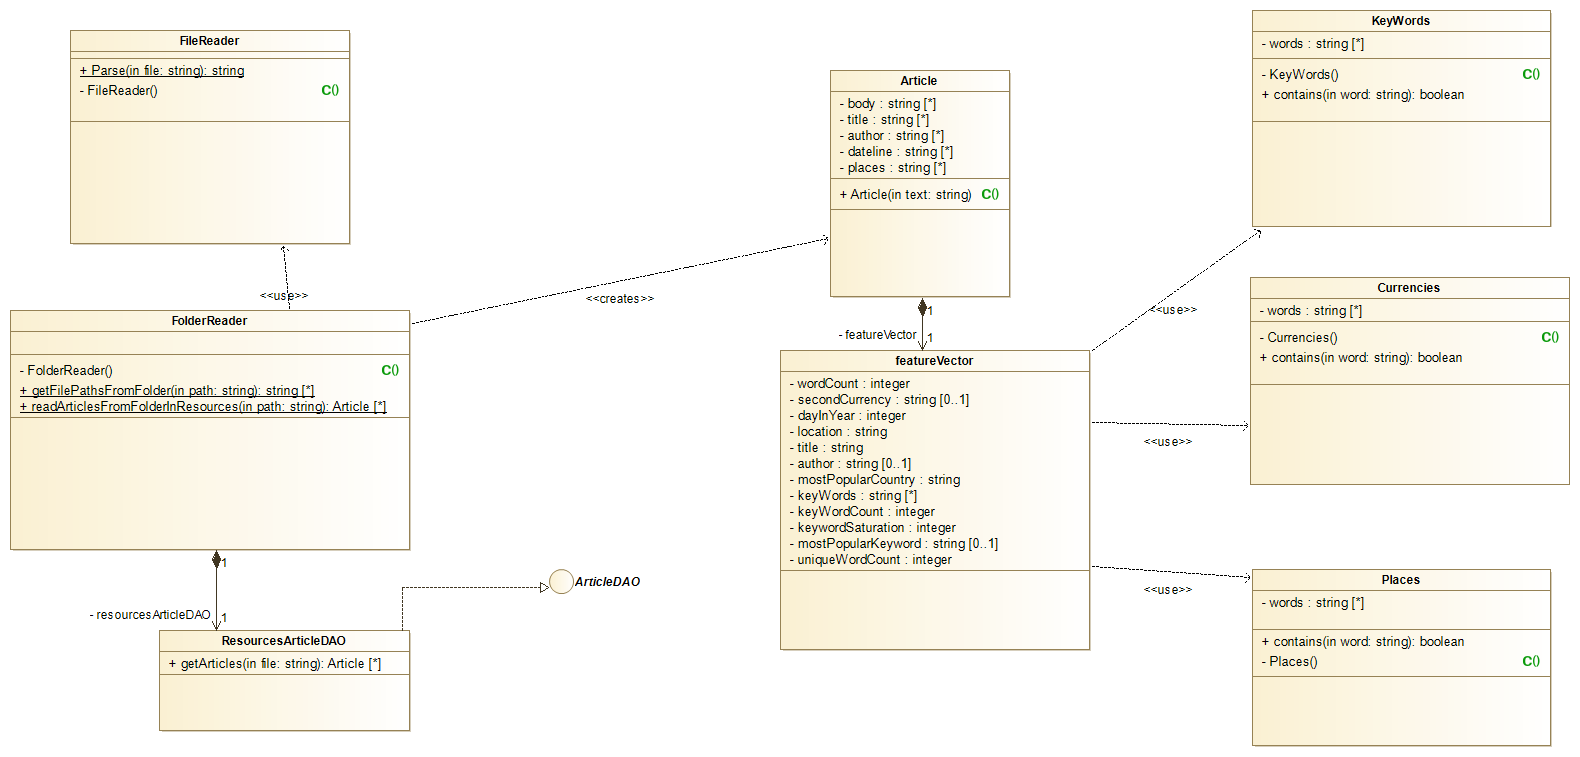
\includegraphics[width=14cm]{Ekstrakcja.png}
 \vspace{-0.3cm}
 \caption{Diagram klas modułu ekstrakcji cech. }
 \label{rysunek do eksperymentu 1 wariantu 1}
\end{figure}
\newpage

Moduł klasyfikacji oblicza odległości pomiędzy artykułem zadanym a każdym z artykułów ze zbioru trenującego za pomocą jednej z zadanych metryk \cite{dane} : metryki Euklidesowej, metryki Ulicznej, metryki Czebyszewa. Dla cech zapisanych w postaci tekstowej ich odległość jest obliczana za pomocą metody bigramów. W ten sposób tworzone są pary zawierające artykuł i odleglość od zadanego artykułu. Następnie znajdowanych jest k najbliższych sąsiadów dla zadanego artykułu, gdzie poprzez słowo sąsiad rozumiemy artykuł ze zbioru trenującego. Ostatecznie artykuł jest klasyfikowany do klasy, której obiekty najczęściej wystąpiły wśród k najbliższych sąsiadów. 

\begin{figure}[h!]
 \centering
 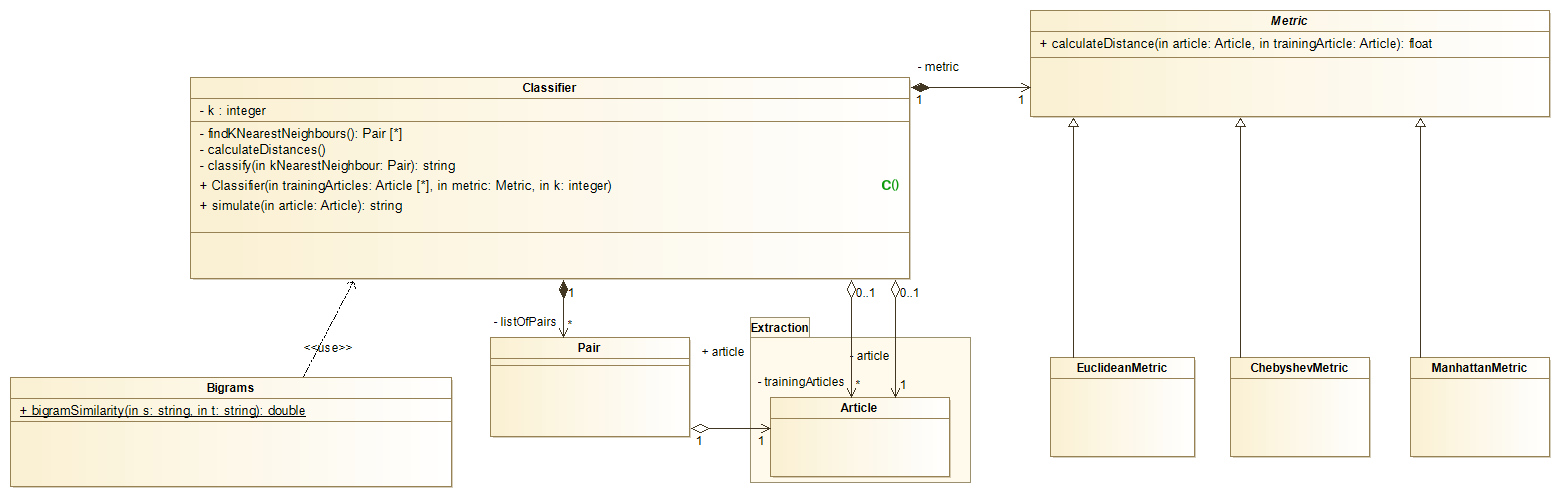
\includegraphics[width=14cm]{Klasyfikator.png}
 \vspace{-0.3cm}
 \caption{Diagram klas modułu klasyfikacji. }
 \label{rysunek do eksperymentu 1 wariantu 1}
\end{figure}

\newpage


%%%%%%%%%%%%%%%%%%%%%%%%%%%%%%%%%%%%%%%%%%%%%%%%%%%%%%%%%%%%%%%%%%
\subsection{Prezentacja wyników, interfejs użytkownika} 

Po uruchomieniu programu użytkownik proszony jest o podanie poprzez konsolę kolejnych parametrów klasyfikacji. Na początku użytkownik podaje wartość parametru k, następnie wybiera jedną z trzech metryk, kolejno podawany jest procent zbioru treningowego w stosunku do zbioru wszystkich tekstów oraz użytkownik może podać cechy tekstów do klasyfikacji. Wybór parametrów w konsoli prezentuje się:

\begin{figure}[h!]
 \centering
 \includegraphics[width=14cm]{Wybor.png}
 \vspace{-0.3cm}
 \caption{Wybór parametrów klasyfikacji przez użytkownika. }
 \label{Wybór parametrów klasyfikacji przez użytkownika. }
\end{figure}

\newpage
Po wprowadzeniu przez użytkownika wszystkich parametrów klasyfikacji, rozpoczynane jest wczytywanie danych oraz wykonanie klasyfikacji. 
\begin{figure}[h!]
 \centering
 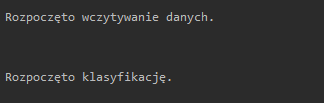
\includegraphics[width=14cm]{srodek.png}
 \vspace{-0.3cm}
 \caption{Wczytywanie danych i klasyfikacja.}
 \label{Wczytywanie danych i klasyfikacja.}
\end{figure}




Po wykonanej klasyfikacji na konsoli wyświetlane są obliczone parametry dla poszczególnych klas klasyfikacji oraz wyliczone parametry dla całego zbioru dokumentów. Dla poszczególnych klas klasyfikacji do obliczonych parametrów zaliczamy liczbę tekstów klasy, liczbę poprawnie zaklasyfikowanych tekstów do rozpatrywanej klasy, liczbę tekstów innych klas zaklasfyfikowanych do rozpatrywanej klasy oraz miary jakości: Precision, Recall, F1. 
\begin{figure}[h!]
 \centering
 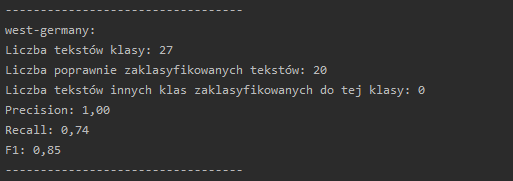
\includegraphics[width=14cm]{wynik_dla _klasy.png}
 \vspace{-0.3cm}
 \caption{Wynik klasyfikacji dla pojedyńczej klasy klasyfikacji - klasa west-germany.}
 \label{Wynik klasyfikacji.}
\end{figure}

Dla całego zbioru dokumentów do obliczonych parametrów zaliczamy liczbę tekstów testowych, liczbę poprawnie zaklasyfikowanych tekstów oraz miary jakości: Accuracy, Precision, Recall, F1. 
  
\begin{figure}[h!]
 \centering
 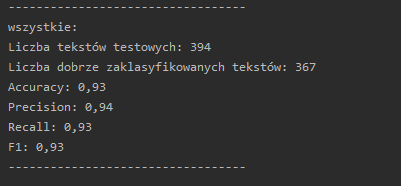
\includegraphics[width=14cm]{wynik.png}
 \vspace{-0.3cm}
 \caption{Wynik klasyfikacji dla całego zbioru dokumentów.}
 \label{Wynik klasyfikacji.}
\end{figure}
\newpage

Do uruchomienia programu wymagana jest wersja Javy: 11. 



%%%%%%%%%%%%%%%%%%%%%%%%%%%%%%%%%%%%%%%%%%%%%%%%%%%%%%%%%%%%%%%%%%
\section{Wyniki klasyfikacji dla różnych parametrów wejściowych}
\subsection{Eksperyment 1 - Wpływ wartości parametru k na miary jakości klasyfikacji}
\label{subsection:ex1}

Eksperymenty zostały rozpoczęte od porównania wyników klasyfikacji dla różnych wartości parametru k.
W tym celu przyjęliśmy nastepujące parametry:
 
\begin{table}[h!]
\caption{Parametry wejściowe dla eksperymentu porównującego różne wartości parametru k. }
\centering
\vspace{0.1cm}
 \begin{tabular}{c c c c}
    \textbf{K} & \textbf{Metryka}   & \textbf{Procent zbioru trenującego}  & \textbf{Wybrane cechy}   \\
\hline
- & Euklidesowa & 80\% &  Wszystkie cechy\\
\end {tabular}
\label {Parametry wejściowe dla eksperymentu porównującego różne wartości parametru k. }
\end{table}

\newpage
\begin{table}[h!]
\caption{Wyniki klasyfikacji dla różnych wartości parametru k. Wartość Nan występująca w tabeli pojawia się, gdy następuje dzielenie przez 0 w Precision. Wartość Nan oznacza, że żaden tekst nie został zaklasyfikowany do tej klasy. Wartość Nan w F1 jest skutkiem wartości Nan w Precision.}
\centering
\vspace{0.1cm}
 \begin{tabular}{c c c c c c c c c c c}

    \textbf{K} & \textbf{1}   & \textbf{2}  & \textbf{3}  & \textbf{4}  & \textbf{5} & \textbf{6}   & \textbf{7}  & \textbf{8}  & \textbf{9}  & \textbf{50} \\

\hline
West-germany Precision 	& 0,12 & NaN & 0,00 & 0,25 & 0,00 & NaN  & NaN & NaN & NaN  & NaN\\
West-germany Recall 		& 0,07 & 0,00 & 0,00 & 0,04 & 0,00 & 0,00 & 0,00 & 0,00 & 0,00 & 0,00\\
West-germany F1		& 0,09 & NaN & 0,00 & 0,06 & 0,00 & NaN  & NaN & NaN & NaN  & NaN \\
\hline
Usa Precision 			& 0,65 & 0,63 & 0,62 & 0,63 & 0,62 & 0,62 & 0,61 & 0,61 & 0,61 & 0,61 \\
Usa Recall				& 0,89 & 0,97 & 0,99 & 1,00 & 1,00 & 1,00 & 0,99 & 1,00 & 1,00 & 1,00 \\
Usa F1			 	& 0,75 & 0,76 & 0,76 & 0,77 & 0,77 & 0,76 & 0,76 & 0,76 & 0,76 & 0,76 \\
\hline
France Precision 		& 0,00 & NaN & NaN & NaN  & 0,00  & NaN & 0,33 & NaN  & NaN & NaN \\
France Recall 			& 0,00 & 0,00 & 0,00 & 0,00 & 0,00 & 0,00 & 0,03 & 0,00 & 0,00 & 0,00 \\
France F1 				& 0,00 & NaN & NaN & NaN  & 0,00 & NaN & 0,06 & NaN  & NaN & NaN\\
\hline
Uk Precision 			& 0,31 & 0,80 & 1,00 & 0,75 & 1,00  & 1,00 & NaN & NaN  & NaN & NaN\\
Uk Recall 				& 0,15 & 0,12 & 0,06 & 0,09 & 0,06 & 0,03 & 0,00 & 0,00 & 0,00 & 0,00\\
Uk F1 				& 0,20 & 0,21 & 0,11 & 0,16 & 0,11  & 0,06 & NaN & NaN  & NaN & NaN \\
\hline
Canada Precision		& 0,17 & 0,00 & 0,00 & 0,00 & NaN & NaN & 1,00 & NaN  & NaN & NaN\\
Canada Recall 			& 0,05 & 0,00 & 0,00 & 0,00 & 0,00 & 0,00 & 0,00 & 0,00 & 0,00 & 0,00 \\
Canada F1 			& 0,08 & 0,00 & 0,00 & 0,00 & NaN & NaN & NaN &  NaN  & NaN & NaN \\
\hline
Japan Precision 		& 0,38 & 0,10 & 0,00 & 0,50 & 0,50  & 0,50 & 1,00 & 1,00 & NaN & NaN \\
Japan Recall 			& 0,07 & 0,02 & 0,00 & 0,02 & 0,02 & 0,02 & 0,02 & 0,02 & 0,00 & 0,00 \\
Japan F1 				& 0,12 & 0,04 & 0,00 & 0,04 & 0,04  & 0,04 & 0,05 & 0,05 & NaN & NaN\\
\hline
Accuracy 				& 0,58 & 0,61 & 0,61 & 0,62 & 0,62 & 0,62 & 0,61 & 0,61 & 0,61 & 0,61 \\
Precision 				& 0,49 & 0,46 & 0,46 & 0,52 & 0,52  & 0,52 & 0,51 &  0,48  & 0,37 & 0,37\\
Recall 				& 0,58 & 0,61 & 0,61 & 0,62 & 0,62 & 0,62 & 0,61 & 0,61 & 0,61 & 0,61  \\
F1 					& 0,53 & 0,52 & 0,53 & 0,57 & 0,56 & 0,56 & 0,56 & 0,54 & 0,46 & 0,46\\

\end {tabular}
\label {t1}
\end{table}

\newpage

\begin{figure}[h!]
 \centering
 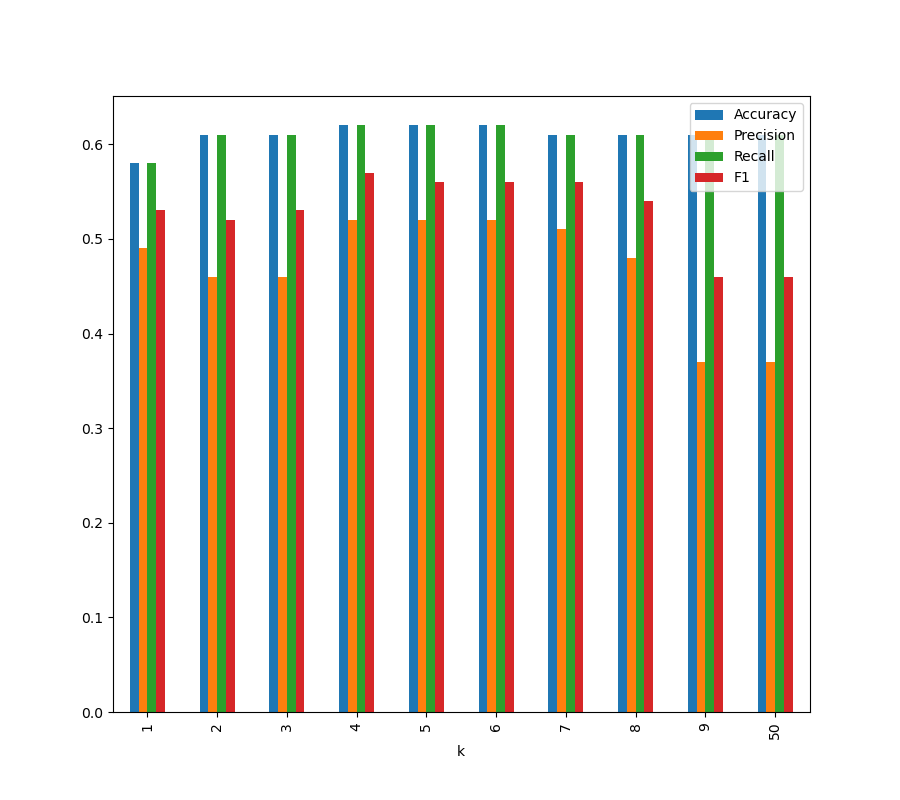
\includegraphics[width=15cm]{wykres_k.png}
 \vspace{-0.3cm}
 \caption{Wykres przedstawia zależność miar Accuracy, Precision, Recall, i F1 od wartości parametru k.}
 \label{wykres1}
\end{figure}

Zmiana parametru k miała największy wpływ na miarę jakości Precision. Najgorszy wynik był dla wartości parametru od 9 wzwyż, a najlepszy dla wartości parametru równego 4. Od wartości k równej 9 wszystkie obiekty zostały zaklasyfikowane do klasy USA, co możemy odczytać z wartości NaN przy obliczaniu precyzji. Wartość taka pojawia się przy dzieleniu przez 0, co oznacza że nie istniał taki obiekt, który zostałby sklasyfikowany do danej klasy. \\



%%%%%%%%%%%%%%%%%%%%%%%%%%%%%%%%%%%%%%%%%%%%%%%%%%%%%%%%%%%%%%%%%%
\subsection{Eksperyment 2 - Wpływ wyboru metryki na miary jakości klasyfikacji}
\label{subsection:ex2}
Następnym eksperymentem jest wykonanie klasyfikacji dla różnych metryk. Pozostałe parametry pozostają niezmienne.\\

Wybrane parametry przedstawione są w poniższej tabeli:
 
\begin{table}[h!]
\caption{Parametry wejściowe dla eksperymentu porównującego różne metryki. }
\centering
\vspace{0.1cm}
 \begin{tabular}{c c c c}
    \textbf{K} & \textbf{Metryka}   & \textbf{Procent zbioru trenującego}  & \textbf{Wybrane cechy}   \\
\hline
4 & - & 90\% &  Wszystkie cechy\\
\end {tabular}
\label {Parametry wejściowe dla eksperymentu porównującego różne metryki. }
\end{table}

\newpage
\begin{table}[h!]
\caption{Wyniki klasyfikacji dla różnych metryk. Wartość Nan występująca w tabeli pojawia się, gdy następuje dzielenie przez 0 w Precision. Wartość Nan oznacza, że żaden tekst nie został zaklasyfikowany do tej klasy. Wartość Nan w F1 jest skutkiem wartości Nan w Precision.}
\centering
\vspace{0.1cm}
 \begin{tabular}{c c c c}

    \textbf{Metryka} & \textbf{Euklidesowa}   & \textbf{Czebyszewa}  & \textbf{Uliczna}  \\

\hline
West-germany Precision 	& 0,00 & 0,00 & 0,20 \\
West-germany Recall 		& 0,00 & 0,00 & 0,04 \\
West-germany F1		& 0,00 & 0,00 & 0,06 \\
\hline
Usa Precision 			& 0,62 & 0,63 & 0,62 \\
Usa Recall				& 0,98 & 0,98 & 0,98 \\
Usa F1			 	& 0,76 & 0,76 & 0,76 \\
\hline
France Precision 		& 0,00 & 0,00 & 0,00 \\
France Recall 			& 0,00 & 0,00 & 0,00 \\
France F1 				& 0,00 & 0,00 & 0,00 \\
\hline
Uk Precision 			& 0,40 & 0,33 & 0,40 \\
Uk Recall 				& 0,06 & 0,09 & 0,06 \\
Uk F1 				& 0,11 & 0,14 & 0,11 \\
\hline
Canada Precision		& 0,00 & 0,00 & NaN \\
Canada Recall 			& 0,00 & 0,00 & 0,00 \\
Canada F1 			& 0,00 & 0,00 & NaN \\
\hline
Japan Precision 		& 0,00 & 0,50 & 0,33 \\
Japan Recall 			& 0,00 & 0,02 & 0,02 \\
Japan F1 				& 0,00 & 0,04 & 0,04 \\
\hline
Accuracy 				& 0,60 & 0,61 & 0,61 \\
Precision 				& 0,41 & 0,47 & 0,46 \\
Recall 				& 0,60 & 0,61 & 0,61 \\
F1 					& 0,49 & 0,53 & 0,53 \\

\end {tabular}
\label {Wyniki klasyfikacji dla różnych metryk.}
\end{table}

\newpage

\begin{figure}[h!]
 \centering
 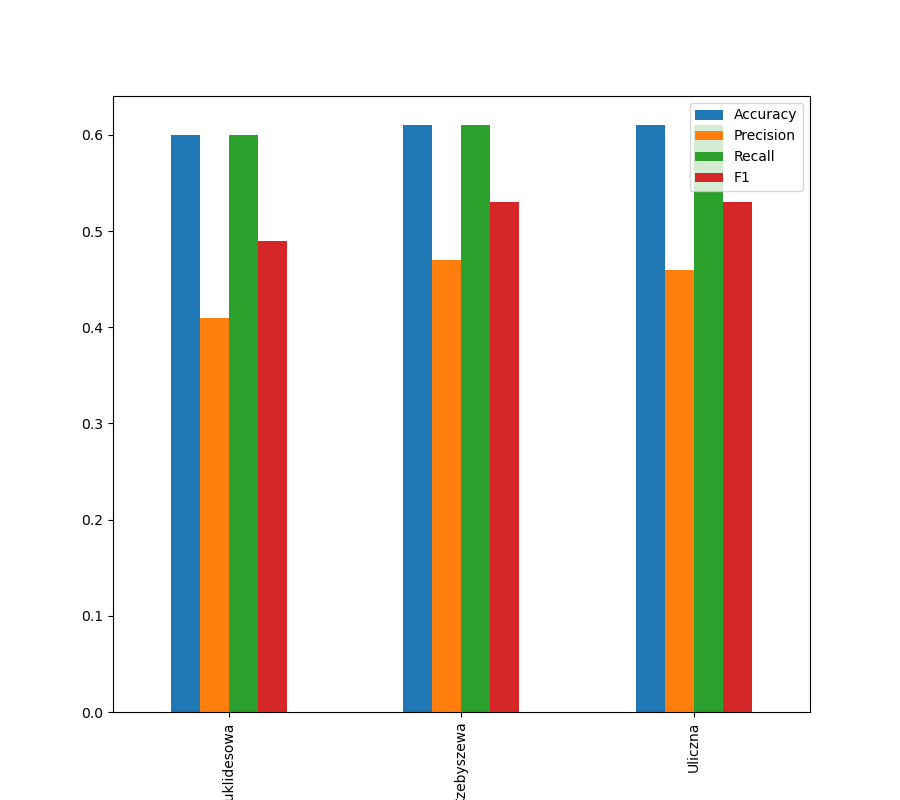
\includegraphics[width=15cm]{wykres_metryka.png}
 \vspace{-0.3cm}
 \caption{Wykres przedstawia zależność miar Accuracy, Precision, Recall, i F1 od metryki.}
 \label{wykres2}
\end{figure}

Metryki uzyskały zbliżone wyniki, spośród nich najlepszą okazała się metryka Czebyszewa, niewiele gorszą, bo z precyzją mniejszą o zaledwie 0.01 była metryka Uliczna. \\



%%%%%%%%%%%%%%%%%%%%%%%%%%%%%%%%%%%%%%%%%%%%%%%%%%%%%%%%%%%%%%%%%%
\subsection{Eksperyment 3 - Wpływ wyboru zestawu cech na miary jakości klasyfikacji}
Następnym eksperymentem jest wykonanie klasyfikacji dla różnych podzbiorów cech. Pozostałe parametry pozostają niezmienne. W tym celu wybieramy sześć różnych zestawów cech. 

Parametry wejściowe dla eksperymentu porównującego różne podzbiory cech:
 
\begin{table}[h!]
\caption{Parametry wejściowe dla eksperymentu porównującego różne podzbiory cech. }
\centering
\vspace{0.1cm}
 \begin{tabular}{c c c c}
    \textbf{K} & \textbf{Metryka}   & \textbf{Procent zbioru trenującego}  & \textbf{Wybrane cechy}   \\
\hline
4 & Euklidesa & 90 & -\\
\end {tabular}
\label {Parametry wejściowe dla eksperymentu porównującego różne podzbiory cech. }
\end{table}

\newpage


\begin{table}[h!]
\caption{Wyniki klasyfikacji dla różnych podzbiorów cech. Wartość Nan występująca w tabeli pojawia się, gdy następuje dzielenie przez 0 w Precision. Wartość Nan oznacza, że żaden tekst nie został zaklasyfikowany do tej klasy. Wartość Nan w F1 jest skutkiem wartości Nan w Precision.}
\centering
\vspace{0.1cm}
 \begin{tabular}{c c c c c c c}

    \makecell{\textbf{Wybrany numer} \\\textbf{zestawu cech}} & \makecell{\textbf{c\textsubscript{1},  c\textsubscript{2}, c\textsubscript{5},} \\\textbf{ c\textsubscript{6}, c\textsubscript{11}}} & \makecell{\textbf{c\textsubscript{3},  c\textsubscript{4},} \\ \textbf{c\textsubscript{5},  c\textsubscript{7}}}  & \textbf{ c\textsubscript{3}}  & \textbf{ c\textsubscript{4}}  & \textbf{ c\textsubscript{3},  c\textsubscript{4}} & 
\makecell{\textbf{c\textsubscript{6}, c\textsubscript{7}, c\textsubscript{8},} \\\textbf{ c\textsubscript{9}, c\textsubscript{10}}} \\

\hline
West-germany Precision 	& 0,00 & 1,00 & 1,00 & 0,71 & 1,00 & 0,22\\
West-germany Recall 		& 0,00 & 0,85 & 0,93 & 0,37 & 0,96 & 0,07\\
West-germany F1		& 0,00 & 0,92 & 0,96 & 0,49 & 0,98 & 0,11\\
\hline
Usa Precision 			& 0,62 & 0,92 & 0,93 & 0,73 & 0,93 & 0,64\\
Usa Recall				& 0,98 & 1,00 & 1,00 & 0,97 & 1,00 & 0,90\\
Usa F1			 	& 0,75 & 0,96 & 0,96 & 0,83 & 0,96 & 0,75\\
\hline
France Precision 		& 0,00 & 1,00 & 1,00 & 0,67 & 1,00 & 0,00\\
France Recall 			& 0,00 & 1,00 & 1,00 & 0,18 & 1,00 & 0,00\\
France F1 				& 0,00 & 1,00 & 1,00 & 0,29 & 1,00 & 0,00\\
\hline
Uk Precision 			& 0,67 & 1,00 & 1,00 & 0,55 & 1,00 & 0,08\\
Uk Recall 				& 0,06 & 0,97 & 0,97 & 0,33 & 0,97 & 0,03\\
Uk F1 				& 0,11 & 0,98 & 0,98 & 0,42 & 0,98 & 0,04\\
\hline
Canada Precision		& 0,00 & 1,00 & 1,00 & 0,75 & 1,00 & 0,31\\
Canada Recall 			& 0,00 & 0,79 & 0,85 & 0,23 & 0,85 & 0,10\\
Canada F1 			& 0,00 & 0,89 & 0,92 & 0,35 & 0,92 & 0,15\\
\hline
Japan Precision 		& 0,00 & 0,97 & 0,97 & 0,76 & 0,97 & 0,67\\
Japan Recall 			& 0,00 & 0,81 & 0,79 & 0,44 & 0,79 & 0,28\\
Japan F1 				& 0,00 & 0,89 & 0,87 & 0,56 & 0,87 & 0,39\\
\hline
Accuracy 				& 0,60 & 0,94 & 0,95 & 0,72 & 0,95 & 0,60\\
Precision 				& 0,43 & 0,95 & 0,95 & 0,72 & 0,96 & 0,52\\
Recall 				& 0,60 & 0,94 & 0,95 & 0,72 & 0,95 & 0,60\\
F1 					& 0,50 & 0,95 & 0,95 & 0,72 & 0,96 & 0,56\\

\end {tabular}
\label {Wyniki klasyfikacji dla różnych podzbiorów cech.}
\end{table}

\begin{figure}[h!]
 \centering
 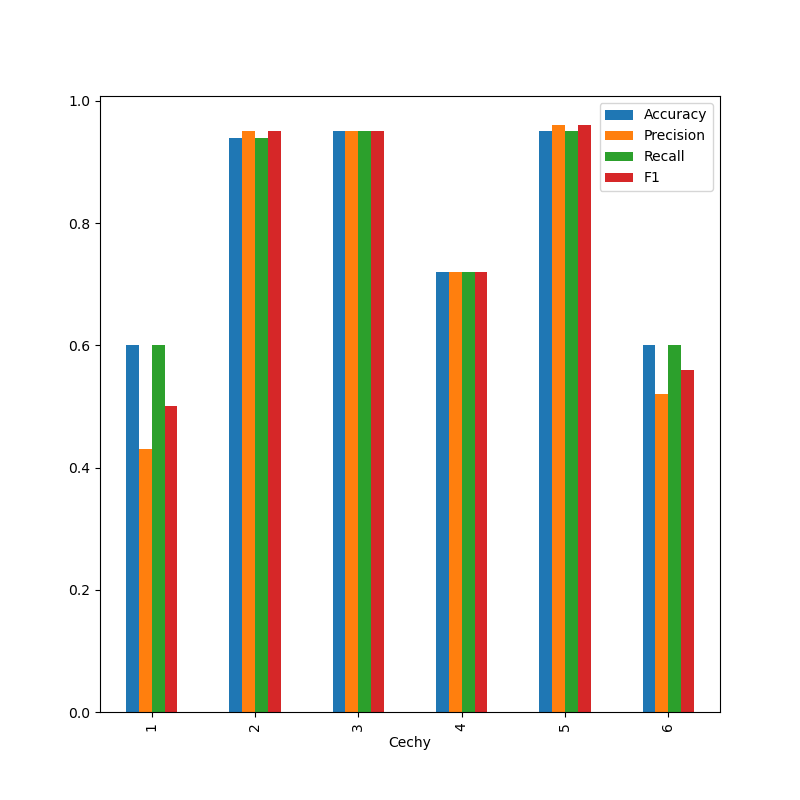
\includegraphics[width=15cm]{wykres_cechy.png}
 \vspace{-0.3cm}
 \caption{Wykres przedstawia zależność miar Accuracy, Precision, Recall, i F1 od podzbioru cech.}
 \label{wykres3}
\end{figure}

\newpage

Po porównaniu zestawów cech odkryliśmy, że najlepszą z cech jest Lokalizacja z tagu \textless Dateline\textgreater. Korzystając tylko z tej jednej cechy uzyskaliśmy prawie najlepsze wyniki, które nieznacznie poprawiło jedynie dodanie do tej cechy Tytułu z tagu \textless Title\textgreater. Dodanie do tych dwu cech autora oraz zbioru cech kluczowych nieznacznie pogorszyło wynik. Inne cechy uzyskały znacznie gorsze wyniki.  \\


%%%%%%%%%%%%%%%%%%%%%%%%%%%%%%%%%%%%%%%%%%%%%%%%%%%%%%%%%%%%%%%%%%
\subsection{Eksperyment 4 - Wpływ wartości proporcji podziału zbioru na miary jakości klasyfikacji}
Ostatnim eksperymentem jest wykonanie klasyfikacji dla różnych wartości proporcji podziału zbioru. Pozostałe parametry pozostają niezmienne.\\ 
Wybrane parametry przedstawione są w poniższej tabeli:
 
\begin{table}[h!]
\caption{Parametry wejściowe dla eksperymentu porównującego różne wartości proporcji podziału zbioru. }
\centering
\vspace{0.1cm}
 \begin{tabular}{c c c c}
    \textbf{K} & \textbf{Metryka}   & \textbf{Procent zbioru trenującego}  & \textbf{Wybrane cechy}   \\
\hline
4 & Euklidesa & - &  c\textsubscript{4}, c\textsubscript{5}\\
\end {tabular}
\label {Parametry wejściowe dla eksperymentu porównującego różne wartości proporcji podziału zbioru. }
\end{table}

\newpage
\begin{table}[h!]
\caption{Wyniki klasyfikacji dla różnych wartości proporcji podziału zbioru. Wartość Nan występująca w tabeli pojawia się, gdy następuje dzielenie przez 0 w Precision. Wartość Nan oznacza, że żaden tekst nie został zaklasyfikowany do tej klasy. Wartość Nan w F1 jest skutkiem wartości Nan w Precision. }
\centering
\vspace{0.1cm}
 \begin{tabular}{c c c c c c}

    \textbf{Proporcje} & \textbf{10}   & \textbf{25}  & \textbf{50}  & \textbf{70}  & \textbf{95}\\

\hline
West-germany Precision 	& NaN & 1,00 & 1,00 & 1,00 & 1,00\\
West-germany Recall 		& 0,00 & 0,48 & 0,48 & 0,74 & 0,96\\
West-germany F1		& NaN & 0,65 & 0,65 & 0,85 & 0,98\\
\hline
Usa Precision 			& 0,68 & 0,78 & 0,86 & 0,90 & 0,96\\
Usa Recall				& 1,00 & 1,00 & 1,00 & 1,00 & 1,00\\
Usa F1			 	& 0,81 & 0,88 & 0,92 & 0,94 & 0,98\\
\hline
France Precision 		& NaN & 1,00 & 1,00 & 1,00 & 1,00\\
France Recall 			& 0,00 & 1,00 & 1,00 & 1,00 & 1,00\\
France F1 				& NaN & 1,00 & 1,00 & 1,00 & 1,00\\
\hline
Uk Precis=sion 			& 0,94 & 0,86 & 1,00 & 1,00 & 1,00\\
Uk Recall 				& 0,97 & 0,97 & 0,97 & 0,97 & 0,97\\
Uk F1 				& 0,96 & 0,91 & 0,98 & 0,98 & 0,98\\
\hline
Canada Precis=sion		& NaN & 1,00 & 1,00 & 0,97 & 1,00\\
Canada Recall 			& 0,00 & 0,41 & 0,59 & 0,74 & 0,87\\
Canada F1 			& NaN & 0,58 & 0,74 & 0,84 & 0,93\\
\hline
Japan Precis=sion 		& 0,83 & 1,00 & 1,00 & 1,00 & 1,00\\
Japan Recall 			& 0,12 & 0,19 & 0,79 & 0,79 & 0,93\\
Japan F1 				& 0,20 & 0,31 & 0,88 & 0,88 & 0,96\\
\hline
Accuracy 				& 0,71 & 0,81 & 0,90 & 0,93 & 0,97\\
Precision 				& 0,59 & 0,85 & 0,91 & 0,93 & 0,98\\
Recall 				& 0,71 & 0,81 & 0,90 & 0,93 & 0,97\\
F1 					& 0,64 & 0,83 & 0,91 & 0,93 & 0,98\\

\end {tabular}
\label {Wyniki klasyfikacji dla różnych wartości proporcji podziału zbioru.}
\end{table}


\begin{figure}[h!]
 \centering
 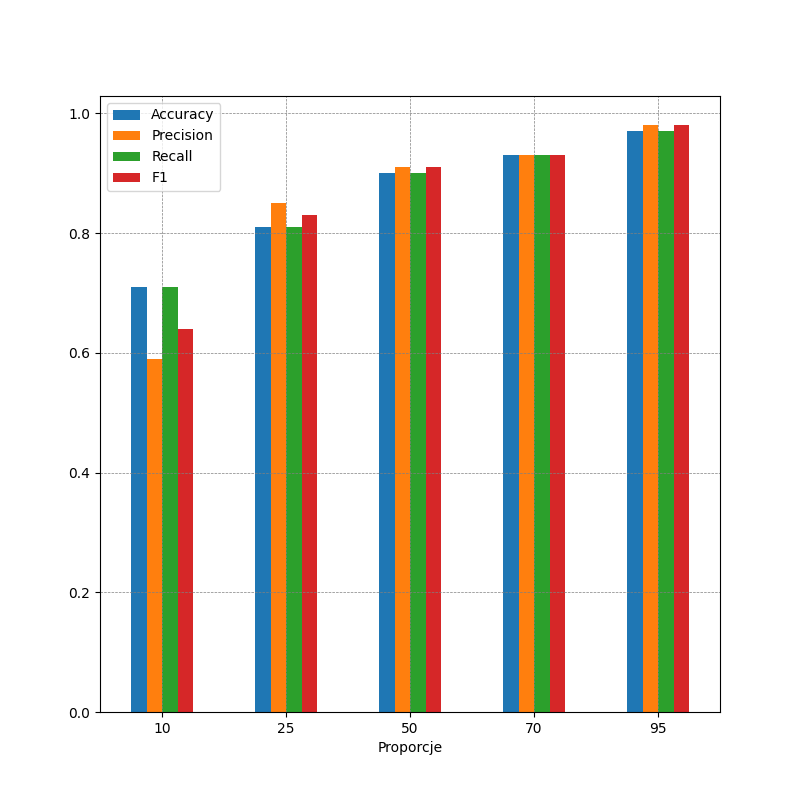
\includegraphics[width=15cm]{wykres_proporcje.png}
 \vspace{-0.3cm}
 \caption{Wykres przedstawia zależność miar Accuracy, Precision, Recall, i F1 od proporcji podziału zbioru.}
 \label{wykres4}
\end{figure}

\newpage


Najlepszą jakość klasyfikacji otrzymano dla proporcji 95 - 5. Zmniejszanie ilości dokumentów w zbiorze treningowym pogarszało jakość klasyfikacji.\\

\newpage


\subsection{Eksperyment 5 - Wpływ wyboru metryki na miary jakości klasyfikacji przy ograniczonym zbiorze cech}
\label{subsection:ex2}
Ze względu na ????????????????????????????????? ponawiamy eksperyment wyboru metryk przy ograniczonym zbiorze cech. \\

Wybrane parametry przedstawione są w poniższej tabeli:
 
\begin{table}[h!]
\caption{Parametry wejściowe dla eksperymentu porównującego różne metryk przy ograniczonym zbiorze cech. }
\centering
\vspace{0.1cm}
 \begin{tabular}{c c c c}
    \textbf{K} & \textbf{Metryka}   & \textbf{Procent zbioru trenującego}  & \textbf{Wybrane cechy}   \\
\hline
4 & - & 90\% &  c\textsubscript{3},  c\textsubscript{4},  c\textsubscript{5},  c\textsubscript{7}, \\
\end {tabular}
\label {Parametry wejściowe dla eksperymentu porównującego różne metryk przy ograniczonym zbiorze cechi. }
\end{table}

\newpage
\begin{table}[h!]
\caption{Wyniki klasyfikacji dla różnych metryk przy ograniczonym zbiorze cech. Wartość Nan występująca w tabeli pojawia się, gdy następuje dzielenie przez 0 w Precision. Wartość Nan oznacza, że żaden tekst nie został zaklasyfikowany do tej klasy. Wartość Nan w F1 jest skutkiem wartości Nan w Precision.}
\centering
\vspace{0.1cm}
 \begin{tabular}{c c c c}

    \textbf{Metryka} & \textbf{Euklidesowa}   & \textbf{Czebyszewa}  & \textbf{Uliczna}  \\

\hline
West-germany Precision 		& 1,00 & 1,00 & 1,00 \\
West-germany Recall 		& 0,85 & 0,04 & 0,93 \\
West-germany F1			& 0,92 & 0,07 & 0,96 \\
\hline
Usa Precision 			& 0,92 & 0,63 & 0,94 \\
Usa Recall				& 1,00 & 1,00 & 1,00 \\
Usa F1			 	& 0,96 & 0,77 & 1,00 \\
\hline
France Precision 			& 1,00 & 0,00 & 1,00 \\
France Recall 			& 1,00 & 0,00 & 1,00 \\
France F1 				& 1,00 & 0,00 & 1,00 \\
\hline
Uk Precision 				& 1,00 & 0,75 & 1,00 \\
Uk Recall 				& 0,97 & 0,09 & 0,97 \\
Uk F1 					& 0,98 & 0,16 & 0,98 \\
\hline
Canada Precision			& 1,00 & NaN & 1,00\\
Canada Recall 			& 0,82 & 0,00 & 0,85 \\
Canada F1 				& 0,90 & NaN & 0,92\\
\hline
Japan Precision 			& 0,97 & 1,00 & 0,97 \\
Japan Recall 				& 0,81 & 0,07 & 0,84 \\
Japan F1 				& 0,89 & 0,13 & 0,90 \\
\hline
Accuracy 				& 0,95 & 0,63 & 0,96 \\
Precision 				& 0,95 & 0,62 & 0,96 \\
Recall 					& 0,95 & 0,63 & 0,96 \\	
F1 					& 0,95 & 0,63 & 0,96 \\

\end {tabular}
\label {Wyniki klasyfikacji dla różnych metryk przy ograniczonym zbiorze cech.}
\end{table}

\newpage

\begin{figure}[h!]
 \centering
 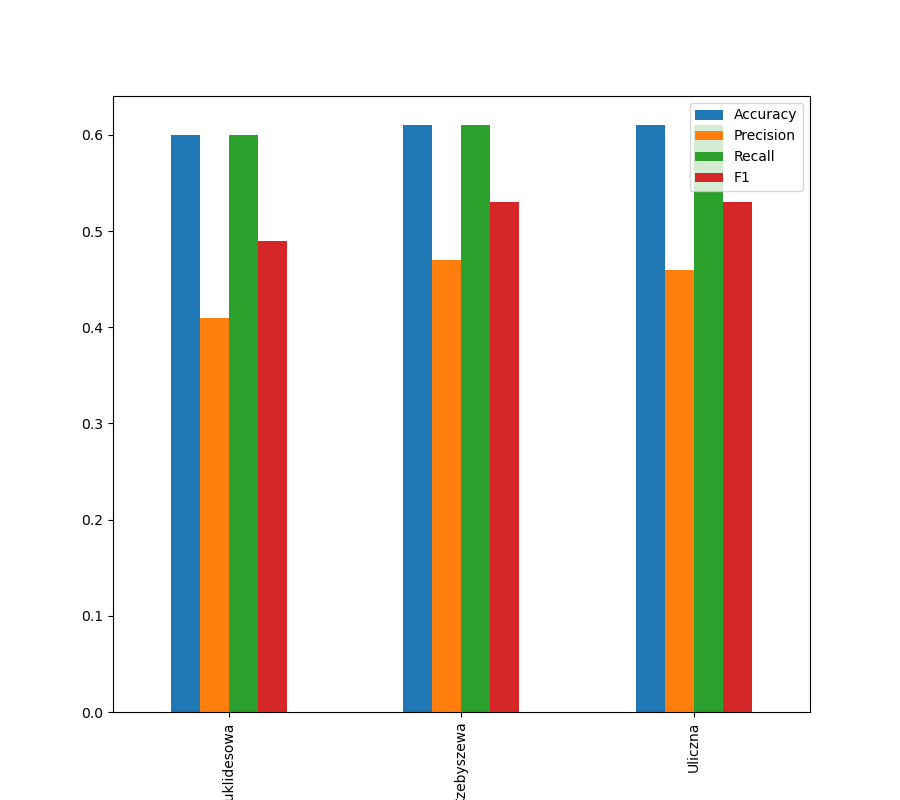
\includegraphics[width=15cm]{wykres_metryka.png}
 \vspace{-0.3cm}
 \caption{Wykres przedstawia zależność miar Accuracy, Precision, Recall, i F1 od metryki przy ograniczonym zbiorze cech.}
 \label{wykres2}
\end{figure}



%%%%%%%%%%%%%%%%%%%%%%%%%%%%%%%%%%%%%%%%%%%%%%%%%%%%%%%%%%%%%%%%%%
\section{Dyskusja, wnioski}

\subsection{Wpływ wartości parametru k na miary jakość klasyfikacji}
W sekcji \ref{subsection:ex1} badającej wpływ wartości parametru k na miary jakość klasyfikacji na podstawie Wykresu \ref{wykres1} zauważamy, że wartość miary accuracy zmienia się wraz ze zmianą wartości paramatru k. Jakość klasyfikacji wzrasta wraz ze wzrostem wartości parametru k, aż do osiągnięcia wartości maksymalnej. Następnie jakość klasyfikacji zaczyna spadać, aż do momentu ustabilizowania się. Po ustabilizowaniu się, zwiększanie parametru k nie wpływa na jakość klasyfikacji. Po przeanalizowaniu wartości precision i recall dla pojedynczych klas w Tabeli \ref{t1} zauważamy, że zmniejszanie się jakości klasyfikacji przy zwiększaniu wartości parametru k jest spowodowane coraz częstszym przyporządkowywaniem elementów do klasy USA. Stabilizowanie się jakości klasyfikacji po wartości progowej parametru k jest wynikiem przyporządkowywania wszystkich elementów do klasy USA. Dla każdej klasy, oprócz klasy USA, wartość recall maleje wraz ze wzrostem parametru k, dla klasy USA wartość miary recall wzrasta aż do osiągnięcia wartości maksymalnej (1.00). Dominacja klasy USA wynika z faktu, że teksty z klasy USA stanowią około 61\% wszystkich klasyfikowanych tekstów. Z tego powodu przy największych wartościach parametru k wartość miary accuracy wynosi okolo 0.61, co wskazuje, że wszystkie teksty zostały zaklasyfikowane do klasy USA. Wartość parametru k ma zauważalny wpływ na jakość klasyfikacji. Dla badanej klasyfikacji oraz dla klasyfikacji o podobnym charakterze istotne jest dobranie odpowiedniej wartości parametru k.

\subsection{Wpływ wyboru metryki na miary jakości klasyfikacji}
W sekcji \ref{subsection:ex2} zostały porównane trzy metryki: metryka Euklidesowa, metryka Czebyszewa, metryka Uliczna. W eksperymencie przyjeliśmy wartość parametru k równą 4, ponieważ w sekcji \ref{subsection:ex1}  ta wartość okazała się być wartością, dla której dla zadanego zbioru dokumentów jakość klasyfikacji była najlepsza. Na podstawie Wykresu \ref{wykres2} zauważamy, że najgorzej wypadającą metryką jest metryka Euklidesowa. Dla metryki Czebyszewa i Ulicznej na podstawie WYkresy \ref{wykres2} nie jesteśmy w stanie określić, która z metryk posiada lepsze wymiki miar jakości klasyfiakcji. Po porównaniu dokładnych wyników w Tabeli \ref{t2}, zauważamy, że metryka Czebyszewa i Uliczna uzyskały niemalże takie same wyniki, a niewielka różnica nastąpiła w miarze precision na korzyść metryki Czebyszewa. 

\section{Braki w realizacji projektu 1.}
Wszystkie obowiązkowe elementy projektu zostały zrealizowane.

%%%%%%%%%%%%%%%%%%%%%%%%%%%%%%%%%%%%%%%%%%%%%%%%%%%%%%%%%%%%%%%%%%
\begin{thebibliography}{0}
\bibitem{dane} R. Tadeusiewicz: Rozpoznawanie obrazów, PWN, Warszawa, 1991.  
\bibitem{niewiadomski08} A. Niewiadomski, Methods for the Linguistic Summarization of Data: Applications of Fuzzy Sets and Their Extensions, Akademicka Oficyna Wydawnicza EXIT, Warszawa, 2008.

\bibitem{wyklad} A. Niewiadomski, ksr-wyklad-2009.pdf, 2009.

\bibitem{tablica} Internet forum. Wikipedia: The Free Encyclopedia, Dostępny w: \url{https://pl.wikipedia.org/wiki/Tablica_pomy%C5%82ek?fbclid=IwAR1yFbhG8HoSicSBnyA43YhpyU0tJiaIpI6ghUdNZvzDhPtMPwAWHtrdPUQ}

\bibitem{teksty} Machine Learning Repository. UCI:, Dostępny w: \url{http://archive.ics.uci.edu/ml/datasets/Reuters-21578+Text+Categorization+Collection}

\end{thebibliography}

\end{document}



